% questions.tex —— 2014 年全国Ⅱ卷（文科） · 题目内容片段（无答案）
% 由 tools/generate_projects.py 依来源总账自 2014/2014_数学真题_全国2文_试题.md 生成，勿手改（改源 MD 后重跑）


\gkpart{数学}

\begin{gktip}
\textbf{来源说明}：本题面依据固定源 PDF 两页 A3 题面逐题转录，原卷印刷页码 905–906。固定源只含试题和作答空白，不附答案或解析；答案和解析均由本库独立复算。

\textbf{图形说明}：第 6、8、18、19、22 题的题面图形在 LaTeX 工程中以 TikZ 矢量源重绘。题面中的图片标记仅为转换器定位这些矢量源的标记，仓库不保存 PNG、JPEG 或 SVG 图形文件。
\end{gktip}

\gkpart{一、选择题}

\begin{question}
\gkti{1}已知集合 $A=\{-2,0,2\}$，$B=\{x\mid x^2-x-2=0\}$，则 $A\cap B=$\mbox{（　　）}

（A）$\varnothing$　　（B）$\{2\}$　　（C）$\{0\}$　　（D）$\{-2\}$

\end{question}
\begin{question}
\gkti{2}$\dfrac{1+3i}{1-i}=$\mbox{（　　）}

（A）$1+2i$　　（B）$-1+2i$　　（C）$1-2i$　　（D）$-1-2i$

\end{question}
\begin{question}
\gkti{3}函数 $f(x)$ 在 $x=x_0$ 处导数存在，若 $p:f'(x_0)=0$；$q:x=x_0$ 是 $f(x)$ 的极值点，则\mbox{（　　）}

（A）$p$ 是 $q$ 的充分必要条件

（B）$p$ 是 $q$ 的充分条件，但不是 $q$ 的必要条件

（C）$p$ 是 $q$ 的必要条件，但不是 $q$ 的充分条件

（D）$p$ 既不是 $q$ 的充分条件，也不是 $q$ 的必要条件

\end{question}
\begin{question}
\gkti{4}设向量 $\boldsymbol a,\boldsymbol b$ 满足 $|\boldsymbol a+\boldsymbol b|=\sqrt{10}$，$|\boldsymbol a-\boldsymbol b|=\sqrt6$，则 $\boldsymbol a\cdot\boldsymbol b=$\mbox{（　　）}

（A）$1$　　（B）$2$　　（C）$3$　　（D）$5$

\end{question}
\begin{question}
\gkti{5}等差数列 $\{a_n\}$ 的公差是 $2$，若 $a_2,a_4,a_8$ 成等比数列，则 $\{a_n\}$ 的前 $n$ 项和 $S_n=$\mbox{（　　）}

（A）$n(n+1)$　　（B）$n(n-1)$　　（C）$\dfrac{n(n+1)}2$　　（D）$\dfrac{n(n-1)}2$

\Needspace{0.4\textheight}
\end{question}
\begin{question}
\gkti{6}如图，网格纸上正方形小格的边长为 $1$（表示 $1\ \mathrm{cm}$），图中粗线画出的是某零件的三视图，该零件由一个底面半径为 $3\ \mathrm{cm}$，高为 $6\ \mathrm{cm}$ 的圆柱体毛坯切削得到，则切削掉的部分的体积与原来毛坯体积的比值为\mbox{（　　）}
\nopagebreak[4]
\begin{center}% 2014 全国卷Ⅱ文科第 6 题：圆柱零件的三视图（方格边长表示 1 cm）。
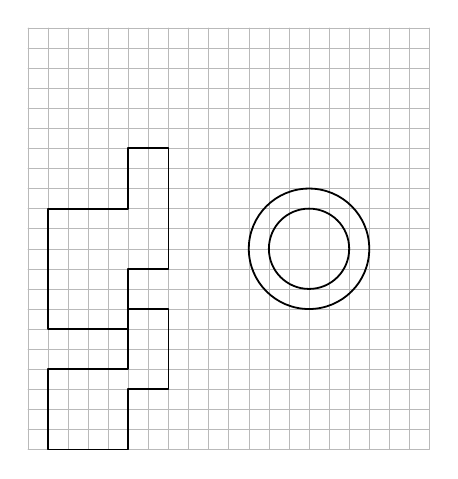
\begin{tikzpicture}[x=2.55mm,y=2.55mm,line cap=round,line join=round]
  % 细灰色方格与题给粗实线分层；原图没有虚线。
  \draw[step=1,gray!55,line width=.18pt] (0,-3) grid (20,18);
  % 左上投影。
  \draw[line width=.65pt] (1,9)--(5,9)--(5,12)--(7,12)--(7,6)--(5,6)--(5,3)--(1,3)--cycle;
  % 左下投影。
  \draw[line width=.65pt] (1,1)--(5,1)--(5,4)--(7,4)--(7,0)--(5,0)--(5,-3)--(1,-3)--cycle;
  % 右上投影：两个同心圆。
  \draw[line width=.65pt] (14,7) circle[radius=3];
  \draw[line width=.65pt] (14,7) circle[radius=2];
\end{tikzpicture}
\end{center}
\nopagebreak[4]
（A）$\dfrac{17}{27}$　　（B）$\dfrac59$　　（C）$\dfrac{10}{27}$　　（D）$\dfrac13$

\end{question}
\begin{question}
\gkti{7}正三棱柱 $ABC-A_1B_1C_1$ 的底面边长为 $2$，侧棱长为 $\sqrt3$，$D$ 为 $BC$ 中点，则三棱锥 $A-B_1DC_1$ 的体积为\mbox{（　　）}

（A）$3$　　（B）$\dfrac32$　　（C）$1$　　（D）$\dfrac{\sqrt3}{2}$

\Needspace{0.4\textheight}
\end{question}
\begin{question}
\gkti{8}执行如图所示的程序框图，如果输入的 $x,t$ 均为 $2$，则输出的 $S=$\mbox{（　　）}
\nopagebreak[4]
\begin{center}% 2014 全国卷Ⅱ文科第 8 题：累加计算程序框图。
\begin{tikzpicture}[font=\footnotesize,>=Stealth,node distance=4mm,line width=.4pt,
  box/.style={draw,minimum height=1.65em,minimum width=7.0em,inner xsep=4pt},
  term/.style={draw,rounded corners=6pt,minimum height=1.65em,inner xsep=8pt},
  io/.style={draw,trapezium,trapezium left angle=70,trapezium right angle=110,
             minimum height=1.65em,inner xsep=4pt},
  dec/.style={draw,diamond,aspect=2.25,inner sep=1.6pt}]
  \node[term] (start) {开始};
  \node[io,below=of start] (input) {输入 $x,t$};
  \node[box,below=of input] (init) {$M=1,\ S=3$};
  \node[box,below=of init] (kinit) {$k=1$};
  \node[dec,below=7mm of kinit] (cond) {$k\leqslant t$};
  \node[box,below left=9mm and 16mm of cond] (calc) {$M=\dfrac{M}{k}x$};
  \node[box,below=of calc] (sum) {$S=M+S$};
  \node[box,below=of sum] (inc) {$k=k+1$};
  \node[io,below right=9mm and 16mm of cond] (output) {输出 $S$};
  \node[term,below=of output] (end) {结束};
  \draw[->] (start)--(input)--(init)--(kinit)--(cond);
  \draw[->] (cond.south west)--node[left] {是}(calc)--(sum)--(inc);
  \draw[->] (inc.west)-| ([xshift=-48mm]cond.west) |- (cond.north);
  \draw[->] (cond.south east)--node[right] {否}(output)--(end);
\end{tikzpicture}
\end{center}
\nopagebreak[4]
（A）$4$　　（B）$5$　　（C）$6$　　（D）$7$

\end{question}
\begin{question}
\gkti{9}设 $x,y$ 满足约束条件

\nopagebreak[4]
\[
\begin{cases}
x+y-1\geqslant0,\\
x-y-1\leqslant0,\\
x-3y+3\geqslant0,
\end{cases}
\]

则 $z=x+2y$ 的最大值为\mbox{（　　）}

（A）$8$　　（B）$7$　　（C）$2$　　（D）$1$

\end{question}
\begin{question}
\gkti{10}设 $F$ 为抛物线 $C:y^2=3x$ 的焦点，过 $F$ 且倾斜角为 $30^\circ$ 的直线交 $C$ 于 $A,B$ 两点，则 $|AB|=$\mbox{（　　）}

（A）$\dfrac{\sqrt{30}}3$　　（B）$6$　　（C）$12$　　（D）$7\sqrt3$

\end{question}
\begin{question}
\gkti{11}若函数 $f(x)=kx-\ln x$ 在区间 $(1,+\infty)$ 单调递增，则 $k$ 的取值范围是\mbox{（　　）}

（A）$(-\infty,-2]$　　（B）$(-\infty,-1]$　　（C）$[2,+\infty)$　　（D）$[1,+\infty)$

\end{question}
\begin{question}
\gkti{12}设点 $M(x_0,1)$，若在圆 $O:x^2+y^2=1$ 上存在点 $N$，使得 $\angle OMN=45^\circ$，则 $x_0$ 的取值范围是\mbox{（　　）}

（A）$[-1,1]$　　（B）$\left[-\dfrac12,\dfrac12\right]$　　（C）$[-\sqrt2,\sqrt2]$　　（D）$\left[-\dfrac{\sqrt2}{2},\dfrac{\sqrt2}{2}\right]$

\end{question}
\gkpart{二、填空题}

\begin{question}
\gkti{13}甲、乙两名运动员各自等可能地从红、白、蓝 $3$ 种颜色的运动服中选择 $1$ 种，则他们选择相同颜色运动服的概率为\gkblank{}。

\end{question}
\begin{question}
\gkti{14}函数 $f(x)=\sin(x+\varphi)-2\sin\varphi\cos x$ 的最大值为\gkblank{}。

\end{question}
\begin{question}
\gkti{15}偶函数 $y=f(x)$ 的图象关于直线 $x=2$ 对称，$f(3)=3$，则 $f(-1)=$\gkblank{}。

\end{question}
\begin{question}
\gkti{16}数列 $\{a_n\}$ 满足 $a_{n+1}=\dfrac1{1-a_n}$，$a_8=2$，则 $a_1=$\gkblank{}。

\end{question}
\gkpart{三、解答题}

\begin{question}
\gkti{17}四边形 $ABCD$ 的内角 $A$ 与 $C$ 互补，$AB=1$，$BC=3$，$CD=DA=2$。

(1) 求 $C$ 和 $BD$；

(2) 求四边形 $ABCD$ 的面积。

\Needspace{0.4\textheight}
\end{question}
\begin{question}
\gkti{18}如图，四棱锥 $P-ABCD$ 中，底面 $ABCD$ 为矩形，$PA\perp$ 平面 $ABCD$，$E$ 为 $PD$ 的中点。
\nopagebreak[4]
\begin{center}% 2014 全国卷Ⅱ文科第 18 题：四棱锥 P-ABCD，E 为 PD 中点。
\begin{tikzpicture}[font=\footnotesize,line width=.45pt,line cap=round,line join=round]
  \coordinate (A) at (0,0);
  \coordinate (B) at (-1.20,-1.70);
  \coordinate (C) at (3.35,-1.70);
  \coordinate (D) at (4.55,0);
  \coordinate (P) at (0,4.25);
  \coordinate (E) at ($(P)!0.5!(D)$);
  \draw (P)--(B)--(C)--(D)--(P);
  \draw (P)--(C) (P)--(E) (E)--(C);
  \draw[dashed] (P)--(A)--(B) (A)--(D) (A)--(C) (A)--(E);
  \node[left] at (P) {$P$};
  \node[above left] at (A) {$A$};
  \node[below left] at (B) {$B$};
  \node[below right] at (C) {$C$};
  \node[right] at (D) {$D$};
  \node[right] at (E) {$E$};
\end{tikzpicture}
\end{center}
\nopagebreak[4]
(1) 证明：$PB\parallel$ 平面 $AEC$；

(2) 设 $AP=1$，$AD=\sqrt3$，三棱锥 $P-ABD$ 的体积 $V=\dfrac{\sqrt3}{4}$，求 $A$ 到平面 $PBC$ 的距离。

\par\medskip

*以下续自固定源 PDF 第 2 页（印刷页 906）。*

\Needspace{0.4\textheight}
\end{question}
\begin{question}
\gkti{19}某市为了考核甲、乙两部门的工作情况，随机访问了 $50$ 位市民，根据这 $50$ 位市民对这两部门的评分（评分越高表明市民的评价越高），绘制茎叶图如下：
\nopagebreak[4]
\begin{center}% 2014 全国卷Ⅱ文科第 19 题：甲、乙部门评分的背靠背茎叶图。
% 左叶保留题面从左至中茎的降序，右叶保留题面的升序。
\begin{tikzpicture}[font=\footnotesize,baseline=(current bounding box.center)]
  \node[anchor=base] at (-3.7,1.25) {甲部门};
  \node[anchor=base] at (3.7,1.25) {乙部门};
  \draw (-7.0,1.00)--(7.0,1.00);
  \draw (-.42,1.55)--(-.42,-7.25);
  \draw (.42,1.55)--(.42,-7.25);
  \foreach \y/\stem/\leftleaves/\rightleaves in {
    0/3/{}/{5\ 9},
    -1/4/{4}/{0\ 4\ 4\ 8},
    -2/5/{9\ 7}/{1\ 2\ 2\ 4\ 5\ 6\ 6\ 7\ 7\ 7\ 8\ 9},
    -3/6/{9\ 7\ 6\ 6\ 5\ 3\ 3\ 2\ 1\ 1\ 0}/{0\ 1\ 1\ 2\ 3\ 4\ 6\ 8\ 8},
    -4/7/{9\ 8\ 8\ 7\ 7\ 7\ 6\ 6\ 5\ 5\ 5\ 5\ 5\ 4\ 4\ 4\ 3\ 3\ 3\ 2\ 1\ 0\ 0}/{0\ 0\ 1\ 1\ 3\ 4\ 4\ 9},
    -5/8/{6\ 6\ 5\ 5\ 2\ 0\ 0}/{1\ 2\ 3\ 3\ 4\ 5},
    -6/9/{6\ 3\ 2\ 2\ 2\ 0}/{0\ 1\ 1\ 4\ 5\ 6},
    -7/10/{}/{0\ 0\ 0}}
    {\node[anchor=east] at (-.62,\y) {\leftleaves};
     \node at (0,\y) {\stem};
     \node[anchor=west] at (.62,\y) {\rightleaves};}
\end{tikzpicture}
\end{center}
\nopagebreak[4]
\Needspace{5\baselineskip}
为避免转换时丢失题面数据，图中两组叶片及中央双分隔线的语义逐行转录如下（左叶仍按题面从左至中茎的顺序，右叶仍按题面从中茎向右的顺序）：

\nopagebreak[4]
\[
\begin{array}{r||c||l}
\text{\text{甲部门}}&\text{\text{茎}}&\text{\text{乙部门}}\\ \hline
&3&5\,9\\
4&4&0\,4\,4\,8\\
9\,7&5&1\,2\,2\,4\,5\,6\,6\,7\,7\,7\,8\,9\\
9\,7\,6\,6\,5\,3\,3\,2\,1\,1\,0&6&0\,1\,1\,2\,3\,4\,6\,8\,8\\
9\,8\,8\,7\,7\,7\,6\,6\,5\,5\,5\,5\,5\,4\,4\,4\,3\,3\,3\,2\,1\,0\,0&7&0\,0\,1\,1\,3\,4\,4\,9\\
6\,6\,5\,5\,2\,0\,0&8&1\,2\,3\,3\,4\,5\\
6\,3\,2\,2\,2\,0&9&0\,1\,1\,4\,5\,6\\
&10&0\,0\,0
\end{array}
\]

(1) 分别估计该市的市民对甲、乙两部门评分的中位数；

(2) 分别估计该市的市民对甲、乙两部门的评分高于 $90$ 的概率；

(3) 根据茎叶图分析该市的市民对甲、乙两部门的评价。

\end{question}
\begin{question}
\gkti{20}设 $F_1,F_2$ 分别是椭圆 $C:\dfrac{x^2}{a^2}+\dfrac{y^2}{b^2}=1\ (a>b>0)$ 的左、右焦点，$M$ 是 $C$ 上一点且 $MF_2$ 与 $x$ 轴垂直，直线 $MF_1$ 与 $C$ 的另一个交点为 $N$。

(1) 若直线 $MN$ 的斜率为 $\dfrac34$，求 $C$ 的离心率；

(2) 若直线 $MN$ 在 $y$ 轴上的截距为 $2$，且 $|MN|=5|F_1N|$，求 $a,b$。

\end{question}
\begin{question}
\gkti{21}已知函数 $f(x)=x^3-3x^2+ax+2$，曲线 $y=f(x)$ 在点 $(0,2)$ 处的切线与 $x$ 轴交点的横坐标为 $-2$。

(1) 求 $a$；

(2) 证明：当 $k<1$ 时，曲线 $y=f(x)$ 与直线 $y=kx-2$ 只有一个交点。

\Needspace{0.4\textheight}
\end{question}
\begin{question}
\gkti{22}如图，$P$ 是 $\odot O$ 外一点，$PA$ 是切线，$A$ 为切点，割线 $PBC$ 与 $\odot O$ 相交于点 $B,C$，$PC=2PA$，$D$ 为 $PC$ 的中点，$AD$ 的延长线交 $\odot O$ 于点 $E$。证明：
\nopagebreak[4]
\begin{center}% 2014 全国卷Ⅱ文科第 22 题：切线、割线及 A-D-E 辅助线。
\begin{tikzpicture}[font=\footnotesize,line width=.45pt,line cap=round,line join=round]
  \coordinate (O) at (0,0);
  \coordinate (P) at (-3.000,-1.225);
  \coordinate (B) at (-1.935,-1.420);
  \coordinate (C) at (1.307,-2.013);
  \coordinate (D) at ($(P)!0.5!(C)$);
  \coordinate (A) at (-2.255,.821);
  \coordinate (E) at (-.417,-2.364);
  \draw (O) circle[radius=2.40];
  \draw (P)--(A);
  \draw (P)--(C);
  \draw (A)--(E);
  \fill (O) circle (1.15pt);
  \node[left] at (P) {$P$};
  \node[left] at (A) {$A$};
  \node[below left] at (B) {$B$};
  \node[below right] at (C) {$C$};
  \node[above right] at (D) {$D$};
  \node[below] at (E) {$E$};
  \node[right] at (O) {$O$};
\end{tikzpicture}
\end{center}
\nopagebreak[4]
(1) $BE=EC$；

(2) $AD\cdot DE=2PB^2$。

\end{question}
\begin{question}
\gkti{23}在直角坐标系 $xOy$ 中，以坐标原点为极点，$x$ 轴正半轴为极轴建立极坐标系，半圆 $C$ 的极坐标方程为 $\rho=2\cos\theta$，$\theta\in\left[0,\dfrac\pi2\right]$。

(1) 求 $C$ 的参数方程；

(2) 设点 $D$ 在 $C$ 上，$C$ 在 $D$ 处的切线与直线 $l:y=\sqrt3x+2$ 垂直，根据 (1) 中你得到的参数方程，确定点 $D$ 的坐标。

\end{question}
\begin{question}
\gkti{24}设函数 $f(x)=\left|x+\dfrac1a\right|+|x-a|\ (a>0)$。

(1) 证明：$f(x)\geqslant2$；

(2) 若 $f(3)<5$，求 $a$ 的取值范围。

\end{question}